%!TEX TS-program = xelatex
%!TEX encoding = UTF-8 Unicode

\documentclass[12pt]{article}
\usepackage{geometry}                % See geometry.pdf to learn the layout options. There are lots.
\geometry{a4paper,top=2cm}
\usepackage[parfill]{parskip}    % Activate to begin paragraphs with an empty line rather than an indent
\usepackage{graphicx}
\usepackage{amsmath}
\usepackage{amssymb}
\usepackage{mathtools}
\usepackage{physics}
\newcommand{\be}{\begin{equation}}
\newcommand{\ee}{\end{equation}}
\usepackage[thicklines]{cancel}
\usepackage[colorlinks=true,citecolor=blue,linkcolor=blue,urlcolor=blue]{hyperref}
\usepackage{booktabs}
\usepackage{csquotes}
\usepackage{qcircuit}
\usepackage{circledsteps}
\usepackage{nicefrac}
\usepackage{fontspec,xltxtra,xunicode}
\usepackage{xcolor}
\usepackage{simplewick}
\defaultfontfeatures{Mapping=tex-text}

\newcommand{\polv}{\ensuremath{\updownarrow}}
\newcommand{\polh}{\ensuremath{\leftrightarrow}}
\newcommand{\poldr}{\rotatebox[origin=c]{45}{\ensuremath{\leftrightarrow}}}
\newcommand{\poldl}{\rotatebox[origin=c]{-45}{\ensuremath{\leftrightarrow}}}
\newcommand{\bigzero}{\mbox{\normalfont\Large\bfseries 0}}
\newcommand{\vecrp}{\ensuremath{\vec{r}^{\,\prime}}}
\newcommand{\vecnr}{\ensuremath{\vec{\nabla}_{\!r}}}

\title{Advanced Quantum Mechanics\\Class 13}
%\author{The Author}
\date{September 20, 2022}                                           % Activate to display a given date or no date

\setcounter{section}{5}
\setcounter{subsection}{14}
\setcounter{equation}{12}

\begin{document}
\maketitle

%%% 01 OKAY

\subsection{Quantum computation (continued)}

What is a quantum computer (QC)?
(grosso modo)
\begin{itemize}
\item device operating an qubits (two-level systems)
\item elementary operations are unitary transformations
\item algorithm running on a QC is a sequence of
unitary transformations acting on the qubits
\item input: a given qubit (one or more)
\item output: qubit after the sequence of
unitary transformations \\$\to$
\fbox{need a measurement to be revealed!}
\end{itemize}

Implementation of the operations with \emph{quantum logic gates}.
Create a program (algorithm) composed by 
quantum circuit diagrams (QCD),
read from left to right.
All in the \emph{computational basis}
$\{\ket{0},\ket{1}\}$.

%%% 02 OKAY

Begin construction of a QCD with the circuit wire: \textbf{---------}\\
line with no operator on it, qubit
remains in the initially prepared state

Initial prepared state \(\rightarrow\) ket with label of
the state on the left of
the wire:
\[
\Qcircuit @C=1em @R=.7em {
      \lstick{\ket{\varphi}} & \qw & \qw
}\stackrel{\text{\textit{e.g.}}}{\Rightarrow}
\,
\left\{
\begin{aligned}
\quad\quad\Qcircuit @C=1em @R=.7em {\lstick{\ket{0}} & \qw & \qw}\\
\quad\quad\Qcircuit @C=1em @R=.7em {\lstick{\ket{1}} & \qw & \qw}\\
\end{aligned}
\right.
\]
If more than one qubit, say \emph{n qubits}
\[
\Qcircuit @C=1em @R=.7em {\lstick{\ket{\varphi}} & \qw {/^n} & \qw}
\]

\emph{Operators:} (gates) unary, binary, ternary 
\(\rightarrow\) they act respectively on a single,
two or three qubit state:

\begin{center}
\begin{minipage}{0.33\textwidth}
\Qcircuit @C=3em @R=.7em {
      & \gate{U} & \qw
}
\end{minipage}%
\quad\quad%
\begin{minipage}{0.33\textwidth}
\Qcircuit @C=3em @R=.7em {
     & \multigate{1}{U} & \qw \\
     & \ghost{U} & \qw
}
\end{minipage}%
\quad\quad%
\begin{minipage}{0.33\textwidth}
\Qcircuit @C=3em @R=.7em {
     & \multigate{2}{U} & \qw \\
     & \ghost{U} & \qw \\
     & \ghost{U} & \qw
}
\end{minipage}
\end{center}

\subsubsection{Unary operators/gates}

\begin{enumerate}
\item \emph{X gate}
\be
X=\sigma_{x} = \begin{pmatrix}0 & 1 \\ 1 & 0\end{pmatrix}
\ee
\be
X\ket{0} = \ket{1},\,X\ket{1} = \ket{0}
\ee

%%% 03
\[
\Qcircuit @C=3em @R=.7em {
      & \gate{X} & \qw & \equiv & \quad & \targ & \qw &
}
\]
$\to$ most common, because of its equivalence with mod.~2 addition.
%
\be
\begin{aligned}
|j\rangle  &=|0\rangle,|1\rangle \\ 
X|j\rangle &=|j \oplus 1\rangle \\ 
X|0\rangle &=|1 \% 2\rangle=|1\rangle \\ 
X|1\rangle &=|2 \% 2\rangle=|0\rangle
\end{aligned}
\ee
where $N\%2$ = 0 for $N$ even and 1 for $N$ odd.
%
\item \emph{Y gate}
\be
Y=\sigma_{y} = \begin{pmatrix}0 & -1 \\ i & 0\end{pmatrix}
\ee
%
\item \emph{Z gate}
\be
Z=\sigma_{s} = \begin{pmatrix}1 & 0 \\ 0 & -1\end{pmatrix}
\ee
%
\item \emph{Phase-shift gate}
\be
R_\varphi = \begin{pmatrix}1 & 0 \\ 0 & e^{i\varphi}\end{pmatrix}
\ee
whence \be Z = R_\pi\ee.
%
\item \emph{S gate}
\be
S = R_{\pi/2} = \begin{pmatrix}1 & 0 \\ 0 & i\end{pmatrix}
\ee
%
\item \emph{T gate}
\be
T = R_{\pi/4} = \begin{pmatrix}1 & 0 \\ 0 & e^{i\pi/2}\end{pmatrix},
\ee
notice that one can extract a global $e^{i\pi/8}$ phase, so
\be
R_{\pi/4} = e^{i\pi/8} \begin{pmatrix}e^{-i\pi/8} & 0 \\ 0 & e^{i\pi/8}\end{pmatrix},
\ee
a.k.a. $\pi/8$ gate.

In circuit diagrams:
%
\Qcircuit @C=1em @R=.7em {
     & \gate{X} & \qw 
},\quad%
\Qcircuit @C=1em @R=.7em {
     & \gate{Y} & \qw 
},\quad\ldots,\quad%
\Qcircuit @C=1em @R=.7em {
     & \gate{T} & \qw 
}%
%
%%% 04 OKAY
\item \emph{Hadamard gate:} crucial gate in QC, as
it produces superposition of
states.
\begin{align} 
\Qcircuit @C=1em @R=.7em { & \gate{H} & \qw }\quad\quad
H 
&=\frac{1}{\sqrt{2}}\left(\begin{array}{cc}1 & 1 \\ 
1 & -1\end{array}\right) \\ 
&=\frac{1}{\sqrt{2}}\left(\sigma_{z}+\sigma_{x}\right) 
\end{align}
\be
\begin{aligned} 
\Qcircuit @C=1em @R=.7em {\lstick{\ket{0}} & \gate{H} & \qw }&=&
\frac{1}{\sqrt{2}}(\sigma_z + \sigma_x) \ket{0} =
\frac{1}{\sqrt{2}}(\ket{0}+\ket{1})\\
\Qcircuit @C=1em @R=.7em {\lstick{\ket{1}} & \gate{H} & \qw }&=&
\frac{1}{\sqrt{2}}(\sigma_z + \sigma_x) \ket{1} =
\frac{1}{\sqrt{2}}(\ket{0}-\ket{1})\\
\end{aligned}
\ee
\end{enumerate}

Identity among unary operators (exercise):
\be
\begin{aligned}
HXH &= Z && H^\dagger = H\\ 
HZH &= X && H^2 = I\\ 
HYH &= -Y && \\ 
\end{aligned}
\ee


\subsubsection{Binary operators/gates}

Operate on two qubits. Reminder of convention:
\be
\begin{aligned}
\ket{00} = 	\begin{pmatrix}1\\0\end{pmatrix}\otimes
			\begin{pmatrix}1\\0\end{pmatrix}=
			\begin{pmatrix}1\\0\\0\\0\end{pmatrix},\quad&
%%% 05 OKAY
\ket{01} = 	\begin{pmatrix}1\\0\end{pmatrix}\otimes
			\begin{pmatrix}0\\1\end{pmatrix}=
			\begin{pmatrix}0\\1\\0\\0\end{pmatrix}\\
\ket{10} = 	\begin{pmatrix}0\\1\end{pmatrix}\otimes
			\begin{pmatrix}1\\0\end{pmatrix}=
			\begin{pmatrix}0\\0\\1\\0\end{pmatrix},\quad&
\ket{11} = 	\begin{pmatrix}0\\1\end{pmatrix}\otimes
			\begin{pmatrix}0\\1\end{pmatrix}=
			\begin{pmatrix}0\\0\\0\\1\end{pmatrix}			
\end{aligned}
\ee

%%% \setcounter
\setcounter{equation}{26}
\begin{enumerate}
\setcounter{enumi}{7}
\item SWAP gate: swaps positions, $\ket{01}\to\ket{10}$, $\ket{10}\to\ket{01}$\\
\be
\raisebox{1em}{\Qcircuit @C=3em @R=1.4em {& \qswap & \qw & \\ & \qswap \qwx & \qw &}}
\quad
\text{SWAP} = 
\begin{pmatrix}
1 & 0 & 0 & 0\\
0 & 0 & 1 & 0\\
0 & 1 & 0 & 0\\
0 & 0 & 0 & 1\\
\end{pmatrix}
\ee
%
\item CNOT gate: control NOT, absolutely crucial as
it entangles two qubits.
CNOT on a
two-qubit state:
\begin{itemize}
\item if 1\textsuperscript{st} (control) qubit is $\ket{0}$, 
does nothing to the 2\textsuperscript{nd} (target) qubit.
\item if 1\textsuperscript{st}           qubit is $\ket{1}$, 
        negates the 2\textsuperscript{nd}          qubit:
        $\ket{0} \leftrightarrow \ket{1}$.
\end{itemize}
%%% 06 OKAY
\be
\raisebox{1em}{\Qcircuit @C=3em @R=1.4em %
{& \ctrl{0} & \qw & \\ & \targ \qwx & \qw & \\  & \ustick{X = \sigma_x} & }}
\quad
\text{CNOT} = 
\begin{pmatrix}
I & 0\\
0 & \sigma_x
\end{pmatrix} = 
\begin{pmatrix}
1 & 0 & 0 & 0\\
0 & 1 & 0 & 0\\
0 & 0 & 0 & 1\\
0 & 0 & 1 & 0\\
\end{pmatrix}
\ee
\emph{Exercise:} Show that
\be
(\text{SWAP})_{ij} = (\text{CNOT})_{ij}(\text{CNOT})_{ji}(\text{CNOT})_{ij}
\ee
but notice this is \emph{not} matrix multiplication!
%
\item \emph{CZ gate} -- control-$Z$:
of control qubit is $\ket{1}$
then apply $Z$ to the
target qubit.
\be
\raisebox{1em}{\Qcircuit @C=3em @R=1.4em %
{& \ctrl{0} & \qw & \\ & \gate{Z} \qwx & \qw & }}
\quad
\text{CZ} = 
\begin{pmatrix}
I & 0\\
0 & \sigma_z
\end{pmatrix} = 
\begin{pmatrix}
1 & 0 & 0 & 0\\
0 & 1 & 0 & 0\\
0 & 0 & 1 & 0\\
0 & 0 & 0 & -1\\
\end{pmatrix}
\ee
\[
\raisebox{1em}{\Qcircuit @C=3em @R=1.4em %
{& \ctrl{0} & \qw & \\ & \ctrl{-1} \qwx & \qw & }}
\quad\Leftarrow\quad
\begin{aligned}
&\text{CZ is symmetric: one can}\\
&\text{choose either qubit as}\\
&\text{the control, end result}\\
&\text{is the same.}\\
\end{aligned}
\]
\end{enumerate}

%%% 07 OKAY

\subsubsection{Ternary operators/gates}

These operate on three qubits.

\begin{enumerate}
\setcounter{enumi}{10}
\item \emph{Toffoli gate:} CCNOT, two first qubits are \emph{control} and third qubit is \emph{target}.
\be
\text{CCNOT} = 
\begin{pmatrix}
 I  &  0  &  0  &  0 \\ 
 0  &  I  &  0  &  0 \\ 
 0  &  0  &  I  &  0 \\ 
 0  &  0  &  0  & \sigma_x\\ 
\end{pmatrix}
=
\begin{pmatrix}
1 & 0 & 0 & 0 & 0 & 0 & 0 & 0 \\ 
0 & 1 & 0 & 0 & 0 & 0 & 0 & 0 \\ 
0 & 0 & 1 & 0 & 0 & 0 & 0 & 0 \\ 
0 & 0 & 0 & 1 & 0 & 0 & 0 & 0 \\ 
0 & 0 & 0 & 0 & 1 & 0 & 0 & 0 \\ 
0 & 0 & 0 & 0 & 0 & 1 & 0 & 0 \\ 
0 & 0 & 0 & 0 & 0 & 0 & 0 & 1 \\ 
0 & 0 & 0 & 0 & 0 & 0 & 1 & 0
\end{pmatrix}
\ee
\[
\Qcircuit @C=3em @R=.7em {
     & \ctrl{0}      & \qw \\
     & \ctrl{-1}     & \qw \\
     & \gate{X} \qwx & \qw \\
}
\quad\raisebox{-1em}{=}\quad
\Qcircuit @C=3em @R=.7em {
     & \ctrl{0}   & \qw \\
     & \ctrl{-1}  & \qw \\
     & \targ \qwx & \qw \\
}
\]
\emph{Examples:}
\be
\begin{aligned}
\text{CCNOT} \ket{110} &= \ket{111}\\
\text{CCNOT} \ket{111} &= \ket{110}\\
\text{CCNOT} \ket{010} &= \ket{010}
\end{aligned}
\ee

%%% 08 OKAY

\item \emph{Fredkin gate:} CSWAP, first qubit is control and second and third qubits are target.
If control is $\ket{0}$: do nothing.
If control is $\ket{1}$: swap the last two (not each one).
\be
\text{CSWAP} = 
\begin{pmatrix}
1 & 0 & 0 & 0 & 0 & 0 & 0 & 0 \\ 
0 & 1 & 0 & 0 & 0 & 0 & 0 & 0 \\ 
0 & 0 & 1 & 0 & 0 & 0 & 0 & 0 \\ 
0 & 0 & 0 & 1 & 0 & 0 & 0 & 0 \\ 
0 & 0 & 0 & 0 & 1 & 0 & 0 & 0 \\ 
0 & 0 & 0 & 0 & 0 & 0 & 1 & 0 \\ 
0 & 0 & 0 & 0 & 0 & 1 & 0 & 0 \\ 
0 & 0 & 0 & 0 & 0 & 0 & 0 & 1
\end{pmatrix}
\ee
Examples:
\be
\begin{aligned}
\text{CSWAP}\ket{110} &= \ket{101}\\
\text{CSWAP}\ket{101} &= \ket{110}
\end{aligned}
\ee
\end{enumerate}

These are one set (among others) that one can use
for whatever computation in a QC.
Now, to extract information,
one needs a measurement, denote it by
\[
\Qcircuit @C=3em @R=.7em {
     & \meter     & \qw
}
\]

%%% 09 OKAY

\subsubsection{Example quantum circuits}

\emph{Example:} let us use a combination of these
operators in a quantum circuit to clone
two known orthogonal states \(|\varphi\rangle\) and \(J \psi\rangle\)
\begin{itemize}
\item consider as states to be cloned:
\be
\begin{aligned}
|\varphi\rangle&=\frac{1}{\sqrt{2}}(|0\rangle+|1\rangle),\quad
|\psi\rangle&=\frac{1}{\sqrt{2}}(|0\rangle-|1\rangle)
\end{aligned}
\ee
%
\item we use these as control qubit and $\ket{0}$ as
target qubit and pass the combined states
through a quantum circuit. The combined
states are:
\be
\begin{aligned}
\ket{\varphi}\ket{0}&=\frac{1}{\sqrt{2}}(\ket{00}+\ket{10}),\quad
\ket{\psi}\ket{0}   &=\frac{1}{\sqrt{2}}(\ket{00}-\ket{10})
\end{aligned}
\ee
%
\item the quantum circuit that does the job is
composed of three Hadamard gates and one CNOT gate:
\[
\Qcircuit @C=3em @R=.7em {
\lstick{\ket{\varphi},\ket\psi} %
 & \gate{H} & \ctrl{0}   & \gate{H} & \qw\\
\lstick{\ket{0}} %
 & \qw      & \targ \qwx & \gate{H} & \qw
}
\]
%
\[
\boxed{
\begin{gathered}
\text{Use of the \emph{same} circuit}\\
\text{to clone }\ket{\varphi},\ket{\psi}
\end{gathered}
}
\]
%
\be
\ket{\varphi}\ket{0}\longrightarrow\ket{\varphi}\ket{\varphi},\quad
\ket{\psi}\ket{0}\longrightarrow\ket{\psi}\ket{\psi},\,
\ee
%
%%% 10 OKAY
\item start with $\ket{\varphi}$:
\begin{itemize}
\item first step: 
pass $\ket{\varphi}\ket{0}$ through
the first Hadamard gate:
\be
\begin{gathered}
\ket{\varphi}\ket{0} = \frac{1}{\sqrt{2}} (\ket{00}+\ket{10})\\
\stackrel{H}{\longrightarrow}
\frac{1}{\sqrt{2}}
\left[
\frac{1}{\sqrt{2}}(\ket{0}+\cancel{\ket{1}})\ket{0} +
\frac{1}{\sqrt{2}}(\ket{0}-\cancel{\ket{1}})\ket{0}
\right]\\
= \ket{00}
\end{gathered}
\ee
\item second step:
pass $\ket{00}$ through the CNOT gate:
\be
\ket{00} \stackrel{\text{CNOT}}{\longrightarrow} \ket{00}
\ee
\item third step: pass $\ket{00}$ through the two $H$ gates:
\be
\begin{gathered}
\ket{00} \stackrel{H^{1},H^{2}}{\longrightarrow} 
\frac{1}{\sqrt{2}}(\ket{0}+\ket{1})
\frac{1}{\sqrt{2}}(\ket{0}+\ket{1})\\
=\ket{\varphi}\ket{\varphi}
\end{gathered}
\ee
\end{itemize}
%
\item next, state $\ket{\psi}$ (let's do this one quickly)
\be
\begin{gathered}
\ket{\psi}\ket{0}
\stackrel{H}{\longrightarrow}
\frac{1}{\sqrt{2}}
\frac{1}{\sqrt{2}}(\cancel{\ket{0}}+\ket{1})\ket{0} +
\frac{1}{\sqrt{2}}(\cancel{\ket{0}}-\ket{1})\ket{0}\\
= \ket{10} \stackrel{\text{CNOT}}{\longrightarrow} \ket{11}\\
\stackrel{H^{1},H^{2}}{\longrightarrow}
\frac{1}{\sqrt{2}}(\ket{0}-\ket{1})
\frac{1}{\sqrt{2}}(\ket{0}-\ket{1})\\
= \ket{\psi}\ket{\psi}
\end{gathered}
\ee
\end{itemize}

%%% 11 OKAY

\emph{Exercise:} 
Design a quantum circuit that clones
the following two orthogonal states:
\be
\begin{aligned}
\ket{\varphi} &= \frac{1}{\sqrt{2}}(\ket{0}+i\ket{1})\\
\ket{\varphi} &= \frac{1}{\sqrt{2}}(\ket{0}-i\ket{1})\\
\end{aligned}
\ee

\emph{Exercise:} show that we can transform the 
computational basis to a Bell State
with the following circuit:
\[
\left.
\raisebox{1em}{\Qcircuit @C=3em @R=.7em {
\lstick{\ket{i}} & \gate{H} & \ctrl{0}   & \qw\\
\lstick{\ket{j}} & \qw      & \targ \qwx & \qw
}}
\right\}
\begin{aligned}
\text{Bell state, when } \ket{i},\ket{j}\\
\text{are } \ket{0} \text{ or } \ket{1}
\end{aligned}
\]
That is:
\be
\begin{aligned}
\ket{00}: \text{CNOT}\,(H)_1 \ket{00} &= \frac{1}{\sqrt 2}(\ket{00}+\ket{11}) = \ket{\Phi^+}\\
\ket{10}: \text{CNOT}\,(H)_1 \ket{10} &= \frac{1}{\sqrt 2}(\ket{00}-\ket{11}) =\ket{\Phi^-}\\
\ket{01}: \text{CNOT}\,(H)_1 \ket{01} &= \frac{1}{\sqrt 2}(\ket{01}+\ket{10}) =\ket{\Psi^+}\\
\ket{11}: \text{CNOT}\,(H)_1 \ket{11} &= \frac{1}{\sqrt 2}(\ket{01}-\ket{10}) = \ket{\Psi^+}
\end{aligned}
\ee

\emph{Exercise:} show that we can transform the 
Bell States to a computation basis
with the following circuit:
\[
\text{Bell state }
\left\{
\raisebox{1em}{\Qcircuit @C=3em @R=.7em {
 & \ctrl{0}    & \gate{H}   & \qw\\
 & \targ \qwx  & \qw        & \qw
}}
\right\}
\ket{i},\ket{j} = \ket{0},\ket{1}
\]
That is:
%%% 12 OKAY
\be
\begin{aligned}
(H)_1\,\text{CNOT} \ket{\Phi^+} &= \ket{00}\\
(H)_1\,\text{CNOT} \ket{\Phi^-} &= \ket{10}\\
(H)_1\,\text{CNOT} \ket{\Psi^+} &= \ket{01}\\
(H)_1\,\text{CNOT} \ket{\Psi^-} &= \ket{11}
\end{aligned}
\ee

\subsection{Information transmission}

\begin{itemize}
\item Entanglement used as resource.
\item Here: dense coding, teleportation.
\end{itemize}

\emph{First note that:}
\begin{itemize}
\item Alice can prepare qubits (e.g. spin-1/2) as she wishes
and send them to Bob. Bob can then measure them
using any axis he likes.
\item There is no advantage of sending qubits
instead of bits. Why?
\item For example: Alice can prepare \(|+, \hat{z}\rangle\) or \(|-, \hat{z}\rangle\),
and Bob can measure about \(\hat{z}\) to infer the
choice Alice made.
\end{itemize}
%%% 13 OKAY 
Therefore, Alice can send \emph{one classical bit}
with each qubit --
she can't do better than this by sending
one qubit a time;
This is true no matter how she prepares
the qubit and no matter how Bob measures it
$\rightarrow$
no more than one bit can be carried
by \emph{one} qubit.

How can one then take advantage of qubits
(superposition principle) to transmit information?

\subsubsection{Dense coding}

A.k.a superdense coding.

Alice sends \emph{two bits} of classical information
to Bob via a \emph{single qubit}.

\begin{center}
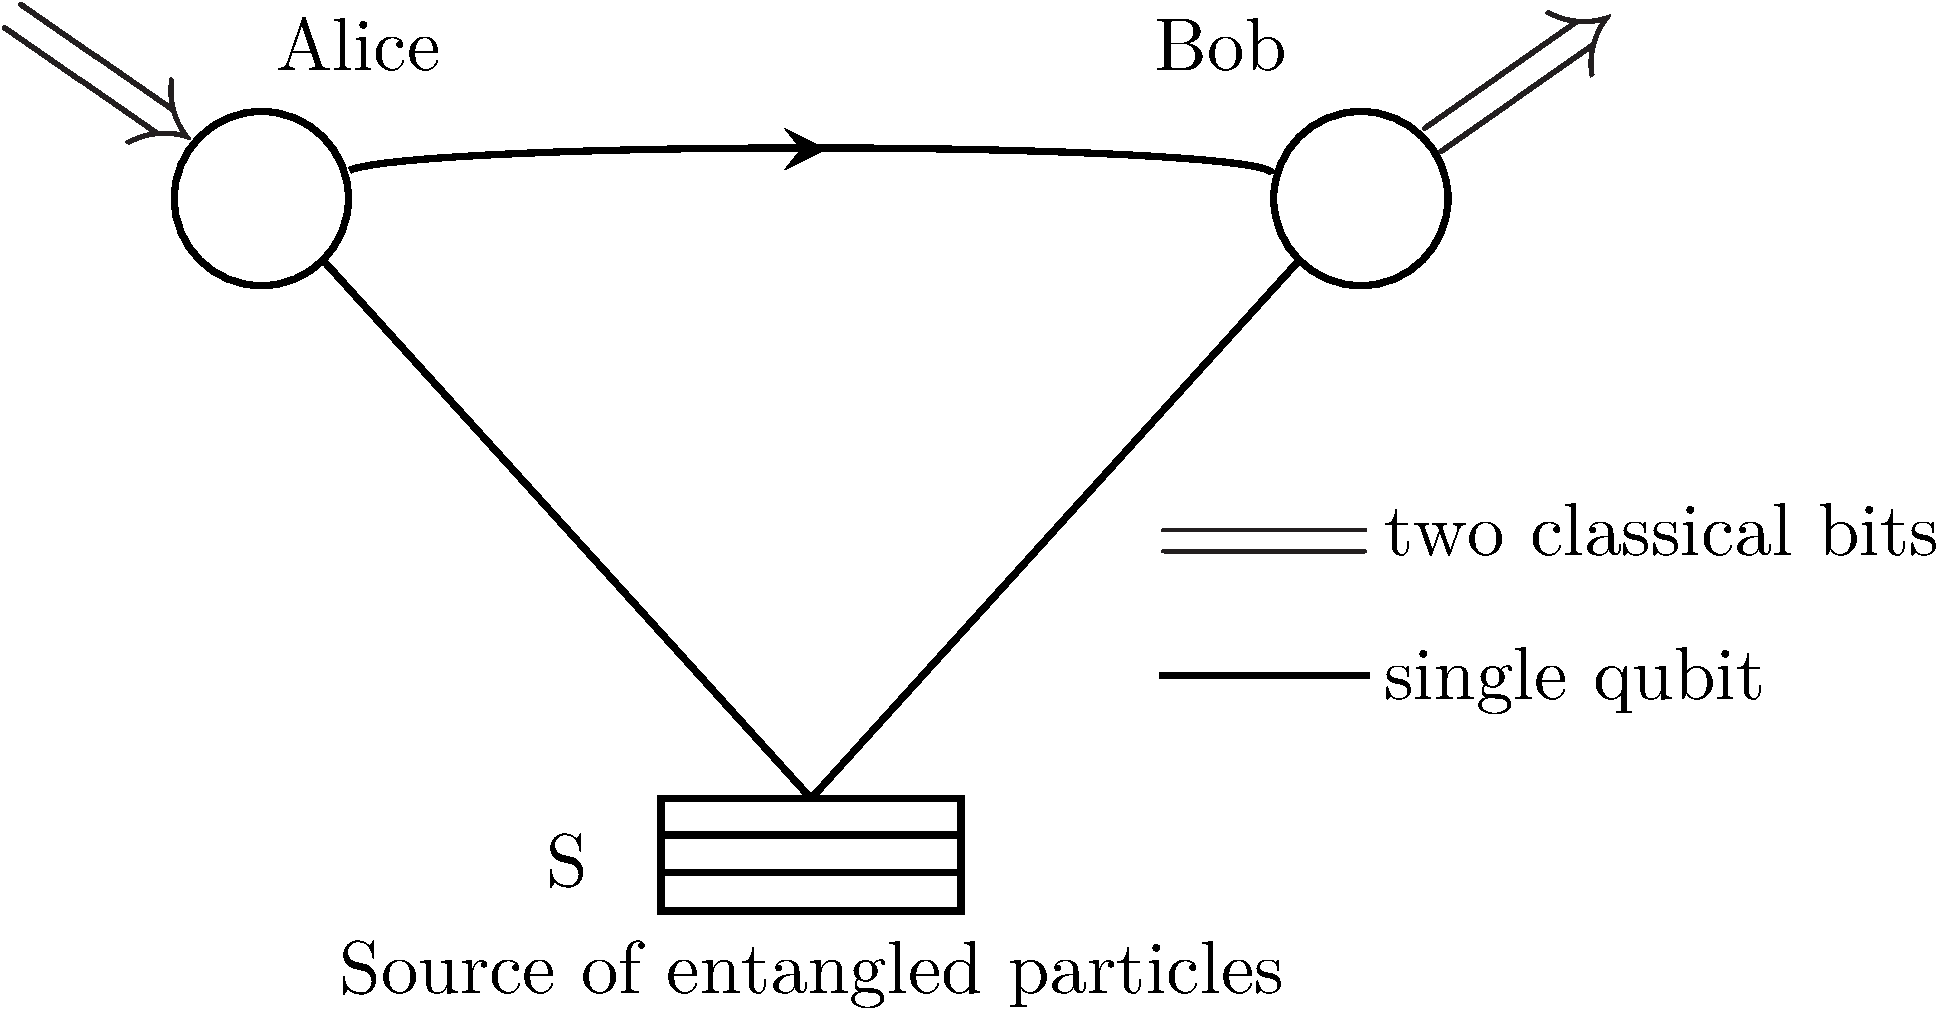
\includegraphics[width=0.6\textwidth]{Figures/AliceAndBobInformation-crop.pdf}
\end{center}

%%% 14 OKAY

A source $S$ generates an entangled pair that
will be shared by Alice and Bob; one member
of the pair goes to Alice and the other to Bob.

\emph{Suppose} this pair is in the $\ket{\Phi^+}$ state:
\be
\ket{\Psi_{AB}} = \frac{1}{\sqrt{2}}(\ket{0_A 0_B} + \ket{1_A 1_B})
\ee
$\rightarrow$
this can be obtained by passing the
state \(|00\rangle\) through the following circuit:
\be
\raisebox{1em}{
\Qcircuit @C=3em @R=.7em{
\lstick{\ket{0}} & \gate{H} & \ctrl{0}   & \qw\\
\lstick{\ket{0}} & \qw      & \targ \qwx & \qw
}}
\quad,\quad
\begin{aligned}
\ket{00} 
&\stackrel{H}{\longrightarrow}          \frac{1}{\sqrt 2}(\ket{00}+\ket{10})\\
&\stackrel{\text{CNOT}}{\longrightarrow}\frac{1}{\sqrt 2}(\ket{00}+\ket{11})
\end{aligned}
\ee

Alice wishes to send one of the following pairs
of bits: \(00,01,10,11\), she will use a protocol
upon which she and Bob agreed earlier.
The protocol consists on a series of unitary
transformations she will apply to her member
of the entangled pair, depending on the
%%% 15 OKAY
pair of bits she wants to send. Then, Alice
sends her qubit to Bob. Then, Bob transforms
the entangled pair to the computational
basis and measures on both members of the pair.
The following set of unitary transformations
does the job:
\be
\begin{aligned}
&1)\,00 \rightarrow I:               &\text{ does nothing}\\
&2)\,01 \rightarrow X =\sigma_{x}:   &\text { rotation of } \pi \text { around } \hat{x}\\
&3)\,10 \rightarrow Z =\sigma_{z}:   &\text { rotation of } \pi \text { around } \hat{z}\\
&4)\,11 \rightarrow ZX =i\sigma_{y}: &\text { rotation of } \pi \text { around } \hat{y} 
\end{aligned}
\ee
By doing so, she transfers \(\left|\Phi_{A B}\right\rangle\) to one of
the following mutually orthogonal states:
\[
\begin{aligned}
1)\,00 \to \ket{\Phi_{AB}}                      &= \frac{1}{\sqrt 2}(\ket{00}+\ket{11})\\
2)\,01 \to \ket{\Phi_{AB}^\prime}               &= \frac{1}{\sqrt 2}(\ket{01}+\ket{10})\\
3)\,10 \to \ket{\Phi_{AB}^{\prime\prime}}       &= \frac{1}{\sqrt 2}(\ket{00}-\ket{11})\\
4)\,11 \to \ket{\Phi_{AB}^{\prime\prime\prime}} &= \frac{1}{\sqrt 2}(\ket{01}-\ket{10})\\
\end{aligned}
\]

%%% 16 OKAY

Next, Alice sends her member of the pair
to Bob \(\Rightarrow\) Bob has the entangled pair
of particles.
Bob transforms the state to the computational
basis and measures on both particles;
result of the measurement reveals
00 or 01 or 10 or 11.
That is, to send two bits Alice needs
to send only one qubit.

\emph{Exercise:} Can Eve intercept the qubit sent by
Alice to Bob and uncover Alice's message?

\subsubsection{Teleportation}

%%% \setcounter
\setcounter{equation}{42}
Alice wants to send to Bob the state of a
spin-1/2 particle (\(\equiv\) particle \(A\)):
\be
\ket{\varphi_A} = \lambda\ket{0_A} + \mu\ket{1_A}
\ee
Alice \emph{does not} know $\lambda$ and $\mu$, and
she \emph{will not} send particle $A$ to Bob.
%%% 17 OKAY
How can she do that?
\begin{enumerate}
\item Alice will use a pair of entangled particles (from a source),
\(B\) and \(C, B\) goes to Alice and \(C\) to Bob.
\item Alice measures on \(A B\), informs (classically)
the result to Bob; Bob receives \((\lambda, \mu)\) through \(C\),
but he does not know \(\lambda\) and \(\mu\).
Fig.~6.13 of Le~Bellac:

\begin{center}
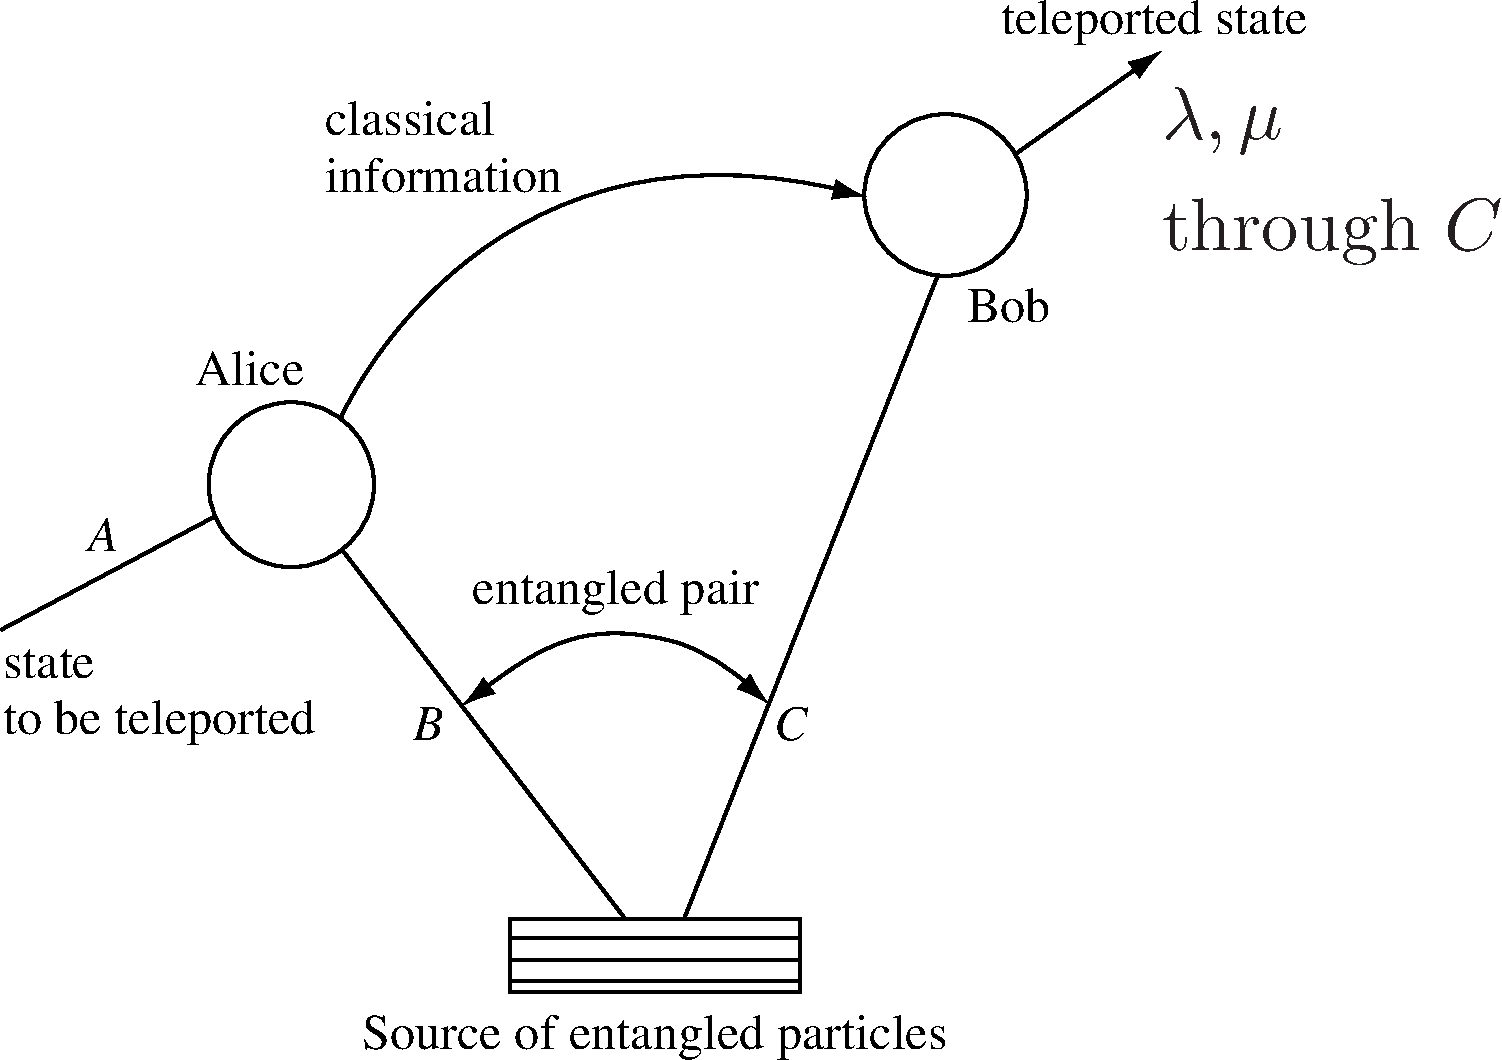
\includegraphics[width=0.6\textwidth]{Figures/AliceAndBobInformation2-crop.pdf}
\end{center}

Particles \(B\) and \(C\) are entangled; suppose as
\be
\ket{\Psi_{BC}} = \frac{1}{\sqrt 2}
(\ket{0_B 0_C}+\ket{1_B 1_C})
\ee
%%% 18 OKAY
so the initial state of the three particles, \(|\Phi_{A B C}\rangle\)
is given by:
\be
\begin{aligned}
\ket{\Phi_{ABC}}
&= (\lambda\ket{0_A} + \mu\ket{1_A})\ket{\Psi_{BC}}\\
&= \frac{\lambda}{\sqrt 2}\ket{0_A} (\ket{0_B0_C} + \ket{1_B1_C})\\
&+ \frac{\mu}    {\sqrt 2}\ket{0_A} (\ket{0_B0_C} + \ket{1_B1_C})
\end{aligned}
\ee
%
\item 
Next, Alice performs a measurement on the $AB$ pair
according to the following circuit:
\[
\Qcircuit @C=3em @R=.7em{
\lstick{\text{qubit }A} & \ctrl{0}     & \gate{H} & \meter\\
\lstick{\text{qubit }B} & \targ \qwx   & \qw      & \meter
}
\] 
\end{enumerate}
$A$ is control, $B$ target: $\ket{\Phi_{ABC}} \stackrel{\text{CNOT}}\longrightarrow \ket{\Phi^\prime_{ABC}}$
\be
\begin{aligned}
\ket{\Phi^\prime_{ABC}}
&= (\text{CNOT})_{AB} \ket{\Phi_{ABC}} \\
&= \frac{\lambda}{\sqrt 2} \ket{0_A}
(\underbrace{\ket{0_B0_C}+\ket{1_B1_C}}_{\Circled{1}})\\
&= \frac{\mu}    {\sqrt 2} \ket{1_A}
(\underbrace{\ket{1_B0_C}+\ket{0_B1_C}}_{\Circled{2}})\\
\end{aligned}
\ee

%%% 19 OKAY
\[
(H)_A \ket{\Phi^\prime_{ABC}} = \ket{\Phi^{\prime\prime}_{ABC}}
\]
whence
\[
\begin{gathered}
\ket{\Phi^{\prime\prime}_{ABC}} = 
\frac{\lambda}{\sqrt 2}
\left(
H\ket{0_A}(\Circled{1})
\right)
+
\frac{\mu}{\sqrt 2}
\left(
H\ket{1_A}(\Circled{2})
\right)\\
=
\frac{\lambda}{\sqrt 2}\frac{1}{\sqrt 2}(\ket{0_A} + \ket{1_A})(\ldots) +
\frac{\mu}    {\sqrt 2}\frac{1}{\sqrt 2}(\ket{0_A} - \ket{1_A})(\ldots) +
\end{gathered}
\]
Now we suppress indices $ABC$, and just use the order $\ket{ABC}$
\be
\begin{aligned}
\ket{\Phi^{\prime\prime}_{ABC}}
&= \frac{\lambda}{2} (\ket{000} + \ket{011} + \ket{100} + \ket{111})\\
&+ \frac{\mu}{2}     (\ket{010} + \ket{001} - \ket{110} + \ket{101})\\
&= \frac{1}{2} \ket{00} (\lambda\ket{0} + \mu\ket{1}) 
 + \frac{1}{2} \ket{01} (\lambda\ket{1} + \mu\ket{0})\\
&+ \frac{1}{2} \ket{10} (\lambda\ket{0} - \mu\ket{1}) 
 + \frac{1}{2} \ket{11} (\lambda\ket{1} - \mu\ket{0})\\
\end{aligned}
\ee
Alice measures on $\ket{AB}$: she can find
\be
\ket{00} \text { or }
\ket{01} \text { or }
\ket{10} \text { or }
\ket{11}
\ee
whence Bob receives
\[
\lambda\ket{0} + \mu\ket{1} \text { or }
\lambda\ket{1} + \mu\ket{0} \text { or }
\lambda\ket{0} - \mu\ket{1} \text { or }
\lambda\ket{1} - \mu\ket{0} 
\]

To recover Alice's original state, Bob needs to
make appropriate operations on his qubit \((\equiv C)\):
\begin{itemize}
\item if Alice tells him that she obtained $\ket{00}$,
he does nothing;
%%% 20 OKAY
\item if Alice tells him that she obtained $\ket{01}$,
he needs to apply $X = \sigma_x$;
\be
X(\lambda\ket{1} + \mu\ket{0}) = \lambda\ket{1} + \mu\ket{0}
\ee
%
\item if Alice tells him that she obtained $\ket{10}$,
he needs to apply $Z = \sigma_z$;
\[
Z(\lambda\ket{0} - \mu\ket{1}) = \lambda\ket{0} + \mu\ket{1}
\]
\end{itemize}
etc.

\emph{Note that:}
\begin{enumerate}
\item \(\lambda\) and \(\mu\) are not measured and \(\left|\varphi_{A}\right\rangle\) is destroyed
by Alice's measurement \(\Rightarrow\) no cloning happened.
\item Bob only gets to ``know'' the state of particle $C$
after Alice's call $\Rightarrow$ information transmitted classically.
\item Particle $A$ is not transported (no matter transport).
\end{enumerate}



\end{document}